% Generado por model/metricas.py - requiere \usepackage{pgfplots}
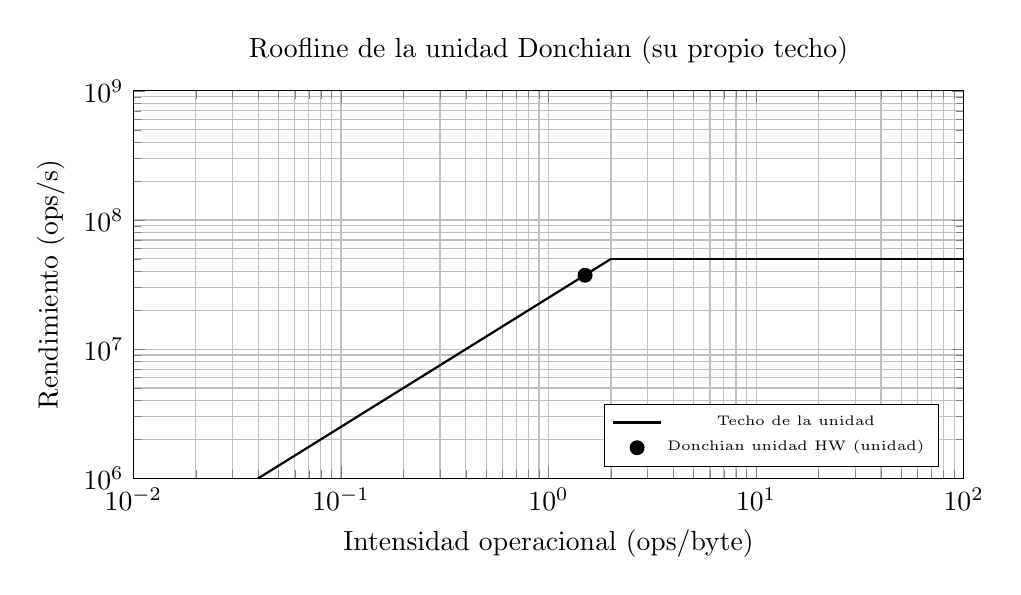
\begin{tikzpicture}
\begin{axis}[
  xmode=log, ymode=log,
  xlabel={Intensidad operacional (ops/byte)}, ylabel={Rendimiento (ops/s)},
  title={Roofline de la unidad Donchian (su propio techo)}, legend pos=south east, legend style={font=\tiny},
  xmin=0.01, xmax=100, ymin=1e+06, ymax=1e+09, grid=both,
  width=\linewidth, height=6.5cm]
\addplot[thick, black, domain=0.01:2, samples=2] {2.5e+07*x};
\addplot[thick, black, domain=2:100, samples=2, forget plot] {5e+07};
\addlegendentry{Techo de la unidad}
\addplot[only marks, mark=*, mark size=2.5pt] coordinates {(1.5,3.73506e+07)};
\addlegendentry{Donchian unidad HW (unidad)}
\end{axis}
\end{tikzpicture}
